%% generato automaticamente da tools/build_tex.py --- non modificare
\chapter{Novantatré modi di guardare $\mathrm{e}$}
\label{cap:e}
\quaderno{e.dfw}{27 Aug 2010}{93}

Agosto 2010, il quaderno più lungo dopo i due gemelli su trigonometria. È una lunga esplorazione attorno al numero di Nepero, condotta con un metodo preciso: prendere la definizione classica $\left(1+\tfrac1x\right)^x$ e romperla in tutti i modi possibili per vedere che cosa resiste. Alcune modifiche distruggono il limite, altre lo lasciano intatto, altre ancora lo spostano in modo controllato. Alla fine il quaderno arriva, senza dichiararlo, alla formula di Eulero.

\section{Che cosa succede se si sottrae un infinitesimo}

Le prime espressioni introducono una perturbazione $\varepsilon$ nella base del limite fondamentale. È lo stesso $\varepsilon$ del quaderno del 2009 (capitolo~\ref{cap:teoria}), qui messo alla prova su un limite notevole.

\begin{espr}{1}{Lim(User,x)}{}
\[
\lim_{x \to \infty} \left(1 + \frac{1}{x} - \varepsilon\right)^{x}
\]
\end{espr}
La base tende a $1-\varepsilon$, un numero minore di uno; elevato a un esponente che diverge, il risultato collassa.

\begin{espr}{2}{Simp(Lim(User,x))}{}
\[
\infty^{\ln\!\left(1 - \varepsilon\right)}
\]
\end{espr}
La scrittura di Derive è formale ma corretta nel segno: $\ln(1-\varepsilon)$ è negativo, e $\infty$ elevato a un esponente negativo vale zero.

\begin{espr}{3}{User}{}
\[
\lim_{x \to \infty} \left(1 + \frac{1}{x} - \frac{1}{99999999999\, x}\right)^{x}
\]
\end{espr}
Ora la perturbazione decresce come $1/x$: è dello stesso ordine del termine che genera $\mathrm{e}$, e quindi conta.

\begin{espr}{4}{Simp(\#3)}{}
\[
\mathrm{e}^{\frac{99999999998}{99999999999}}
\]
\end{espr}
Il risultato è $\mathrm{e}$ elevato a un esponente pochissimo minore di uno.

\begin{espr}{5}{User}{}
\[
\lim_{x \to \infty} \left(1 + \frac{1}{x} - \frac{1}{k\, x}\right)^{x}
\]
\end{espr}
La stessa cosa con un parametro generico al posto del numero di undici cifre.

\begin{espr}{6}{Simp(\#5)}{}
\[
\mathrm{e}^{1 - \frac{1}{k}}
\]
\end{espr}
La formula generale: $\mathrm{e}^{1-1/k}$. Per $k=1$ vale $1$, per $k\to\infty$ tende a $\mathrm{e}$.

\begin{espr}{7}{Lim(User,}{}
\[
\lim_{\varepsilon \to 0} \left(1 + \frac{1}{k\, \varepsilon} - \varepsilon\right)^{\frac{1}{k\, \varepsilon}}
\]
\end{espr}
Si scambiano i ruoli: ora è $\varepsilon$ a tendere a zero e a comparire anche nell'esponente.

\begin{espr}{8}{Simp(\#7)}{}
\[
\mathrm{?}
\]
\end{espr}
Derive non conclude: il punto interrogativo è la sua risposta quando la forma è indeterminata.

\begin{espr}{9}{User}{}
\[
\lim_{\varepsilon \to 0} \left(1 + \frac{1}{\varepsilon} - \varepsilon\right)^{\frac{1}{\varepsilon}}
\]
\end{espr}
Variante senza il parametro $k$.

\begin{espr}{10}{Simp(\#9)}{}
\[
\mathrm{?}
\]
\end{espr}
Ancora indeterminato.

\begin{espr}{11}{User}{}
\[
\lim_{\varepsilon \to 0} \left(\frac{1}{\varepsilon}\right)^{\ln\!\left(1 - \varepsilon\right)}
\]
\end{espr}
Una forma più semplice della stessa famiglia, questa volta trattabile.

\begin{espr}{12}{Simp(\#11)}{}
\[
1
\]
\end{espr}
Il limite vale $1$: infatti $\ln(1-\varepsilon)\approx-\varepsilon$, e $(1/\varepsilon)^{-\varepsilon}=\mathrm{e}^{-\varepsilon\ln(1/\varepsilon)}\to1$.

\begin{espr}{13}{User}{}
\[
\lim_{x \to \infty} \left(\varepsilon\, x + \frac{1}{x} - \varepsilon\right)^{x}
\]
\end{espr}
Qui $\varepsilon$ moltiplica $x$: la base diverge invece di tendere a uno.

\begin{espr}{14}{Simp(\#13)}{}
\[
\mathbb{S}^{1}\, \infty
\]
\end{espr}
La risposta di Derive dice due cose: il modulo è infinito e la fase è indeterminata. $\mathtt{unit\_circle}$ è il modo del programma di indicare un argomento qualsiasi.


Il risultato di questo primo gruppo è che $\varepsilon$ e $1/x$ non sono intercambiabili. Se la perturbazione è una costante, per quanto piccola, la base tende a $1-\varepsilon<1$ e la potenza $x$-esima annulla tutto. Se invece la perturbazione decresce come $1/x$ — cioè allo stesso ordine del termine che genera $\mathrm{e}$ — il limite resta finito e vale $\mathrm{e}^{1-1/k}$. Fissato $k$, si ottiene un'intera famiglia di valori che interpola fra $1$ e $\mathrm{e}$: per $k=1$ la perturbazione cancella esattamente il termine $1/x$ e il limite è $1$; per $k\to\infty$ si ritrova $\mathrm{e}$.

\section{Aggiungere termini non cambia nulla}

Domanda opposta: e se invece di togliere si aggiunge? Le espressioni seguenti mettono nella base non solo $1/x$ ma anche $1/x^2$, $1/x^3$, e infine tutta la serie geometrica.

\begin{espr}{15}{User}{}
\[
\lim_{x \to \infty} \left(1 + \frac{1}{x} + \frac{1}{x^{2}}\right)^{x}
\]
\end{espr}
Si aggiunge un termine di ordine $1/x^2$.

\begin{espr}{16}{Simp(\#15)}{}
\[
\mathrm{e}
\]
\end{espr}
Il limite non cambia.

\begin{espr}{17}{User}{}
\[
\lim_{x \to \infty} \left(1 + \frac{1}{x} + \frac{1}{x^{2}} + \frac{1}{x^{3}} + \frac{1}{x^{4}}\right)^{x}
\]
\end{espr}
Se ne aggiungono altri due.

\begin{espr}{18}{Simp(\#17)}{}
\[
\mathrm{e}
\]
\end{espr}
Ancora $\mathrm{e}$.

\begin{espr}{19}{Lim(User,x)}{}
\[
\lim_{x \to \infty} \left(\sum_{n=0}^{\infty} \frac{1}{x^{n}}\right)^{x}
\]
\end{espr}
Il caso limite: tutta la serie geometrica $\sum_{n\ge0}x^{-n}$.

\begin{espr}{20}{User}{}
\[
\lim_{x \to \infty} \left(\sum_{n=0}^{9} \frac{1}{x^{n}}\right)^{x}
\]
\end{espr}
Troncata a dieci termini.

\begin{espr}{21}{User}{}
\[
\lim_{x \to \infty} \left(\sum_{n=0}^{99} \frac{1}{x^{n}}\right)^{x}
\]
\end{espr}
Troncata a cento.

\begin{espr}{22}{Simp(\#21)}{}
\[
\mathrm{e}
\]
\end{espr}
Il valore è sempre lo stesso, e si capisce perché: solo il primo termine oltre l'unità sopravvive al limite.


Il limite non si muove: resta $\mathrm{e}$. La ragione è che solo il termine di ordine $1/x$ conta. Se la base è $1+\tfrac1x+O\!\left(\tfrac{1}{x^2}\right)$, il logaritmo vale $\tfrac1x+O\!\left(\tfrac{1}{x^2}\right)$ e moltiplicato per $x$ tende a $1$. Tutto ciò che decresce più in fretta di $1/x$ è invisibile al limite. È il complemento esatto della sezione precedente: là una perturbazione troppo lenta distruggeva il limite, qui una troppo rapida non lo tocca.

\section{Il rischio di sostituire un valore finito}

Un intermezzo che vale come avvertimento. Che cosa succede se in una formula pensata per $x$ grande si sostituisce un valore concreto?

\begin{espr}{23}{User}{}
\[
\left(1 + \frac{1}{100} - 100\right)^{\frac{1}{100}}
\]
\end{espr}
Che cosa dà la formula se si mette $x=100$ dentro una scrittura pensata per $x\to\infty$.

\begin{espr}{24}{Simp(\#23)}{}
\[
\left(\frac{9899}{100}\right)^{\frac{1}{100}}\, \left(-1\right)^{\frac{1}{100}}
\]
\end{espr}
La base è negativa: Derive isola il fattore $(-1)^{1/100}$.

\begin{espr}{25}{User}{}
\[
\left(1 + \frac{1}{999} - 999\right)^{\frac{1}{999}}
\]
\end{espr}
Stessa prova con $x=999$.

\begin{espr}{26}{Simp(\#25)}{}
\[
\left(\frac{997001}{999}\right)^{\frac{1}{999}}\, \left(-1\right)^{\frac{1}{999}}
\]
\end{espr}
Stessa struttura.

\begin{espr}{27}{Approx(\#26)}{}
\[
1.006931633 + 0.003166545996\, \mathrm{i}
\]
\end{espr}
Il valore numerico è complesso, con parte immaginaria piccola ma non nulla: è la determinazione principale della radice centesima di un numero negativo.


La base diventa negativa e la potenza frazionaria esce dai reali. Derive, che lavora con la determinazione principale, restituisce correttamente un numero complesso. Non è un errore del programma: è quello che accade quando si prende una formula asintotica e la si valuta fuori dal suo regime.

\section{Troncare la serie all'indice variabile}

Variante più sottile: sommare la serie geometrica non fino all'infinito ma fino a $n=x$, cioè con un numero di termini che cresce insieme alla variabile.

\begin{espr}{28}{User}{}
\[
\left(\sum_{n=0}^{\infty} \frac{1}{x^{n}}\right)^{x} = \mathrm{e}
\]
\end{espr}
L'affermazione che il quaderno vuole verificare: la serie geometrica al posto del binomio dà ancora $\mathrm{e}$.

\begin{espr}{29}{User}{}
\[
\lim_{x \to \infty} \left(\sum_{n=0}^{x} \frac{1}{x^{n}}\right)^{x}
\]
\end{espr}
Variante con l'estremo superiore della somma legato alla variabile.

\begin{espr}{30}{Simp(User)}{}
\[
1
\]
\end{espr}
\begin{espr}{31}{User}{}
\[
\left(\sum_{n=0}^{x} \frac{1}{x^{n}}\right)^{x}
\]
\end{espr}
La somma parziale scritta esplicitamente.

\begin{espr}{32}{Simp(\#31)}{}
\[
\left(\frac{x^{-x}\, \left(x^{x + 1} - 1\right)}{x - 1}\right)^{x}
\]
\end{espr}
La sua forma chiusa: somma di una geometrica di ragione $1/x$ con $x+1$ termini.

\begin{espr}{33}{Lim(\#32,x)}{}
\[
\lim_{x \to \mathrm{e}} \left(\frac{x^{-x}\, \left(x^{x + 1} - 1\right)}{x - 1}\right)^{x}
\]
\end{espr}
Valutata in $x=\mathrm{e}$.

\begin{espr}{34}{Approx(\#33)}{}
\[
3.254394129
\]
\end{espr}
Circa $3{,}2544$.

\begin{espr}{35}{Lim(\#32,x)}{}
\[
\lim_{x \to \pi} \left(\frac{x^{-x}\, \left(x^{x + 1} - 1\right)}{x - 1}\right)^{x}
\]
\end{espr}
Valutata in $x=\pi$.

\begin{espr}{36}{Approx(User)}{}
\[
3.24219215
\]
\end{espr}
Circa $3{,}2422$. I due valori sono vicini fra loro ma non a $\mathrm{e}$: il troncamento all'indice $x$ cambia la natura del limite.


La forma chiusa $\#32$ è la somma di una progressione geometrica di ragione $1/x$ con $x+1$ termini. Valutata nei due punti notevoli $x=\mathrm{e}$ e $x=\pi$ dà due numeri vicini fra loro e vicini a $\pi$, ma senza un significato particolare: sono le prime due tacche di una curva che il quaderno non prosegue.

\section{La parabola che ha per radici $\mathrm{e}$ e $\pi$}

Cambio di scena. Si costruisce il polinomio di secondo grado più semplice che si annulla nei due numeri, e se ne studiano vertice e integrale.

\begin{espr}{37}{User}{}
\[
y = x^{2} - \left(\pi + \mathrm{e}\right)\, x + \pi\, \mathrm{e}
\]
\end{espr}
Il polinomio di secondo grado con radici $\mathrm{e}$ e $\pi$, scritto per somma e prodotto delle radici.

\begin{espr}{38}{User}{}
\[
x^{2} - \left(\pi + \mathrm{e}\right)\, x + \pi\, \mathrm{e} = 0
\]
\end{espr}
La stessa cosa come equazione.

\begin{espr}{39}{Simp(Solve(\#38,x))}{}
\[
x = \mathrm{e} \;\lor\; x = \pi
\]
\end{espr}
Derive conferma le due radici.

\begin{espr}{40}{Dif(\#37,x)}{}
\[
\frac{\mathrm{d}}{\mathrm{d}x}\!\left[y = x^{2} - \left(\pi + \mathrm{e}\right)\, x + \pi\, \mathrm{e}\right]
\]
\end{espr}
Si deriva per cercare il vertice.

\begin{espr}{41}{Simp(Solve(User,x))}{}
\[
x = \frac{\mathrm{e} + \pi}{2}
\]
\end{espr}
L'ascissa del vertice è la media dei due numeri, $\approx 2{,}930$.

\begin{espr}{42}{User}{}
\[
y = -\frac{\left(\mathrm{e} - \pi\right)^{2}}{4}
\]
\end{espr}
L'ordinata del vertice: metà differenza al quadrato, cambiata di segno.

\begin{espr}{43}{User}{}
\[
\int_{\pi}^{\mathrm{e}} x^{2} - \left(\pi + \mathrm{e}\right)\, x + \pi\, \mathrm{e} \,\mathrm{d}x
\]
\end{espr}
L'integrale fra le due radici, percorso da $\pi$ verso $\mathrm{e}$.

\begin{espr}{44}{User}{}
\[
\frac{\left(\pi - \mathrm{e}\right)^{3}}{3!}
\]
\end{espr}
Il valore, in forma notevole: la differenza al cubo divisa per $3!$.

\begin{espr}{45}{Approx(User)}{}
\[
0.01264232275
\]
\end{espr}
Numericamente circa $0{,}01264$.

\begin{figure}[htbp]
  \centering
  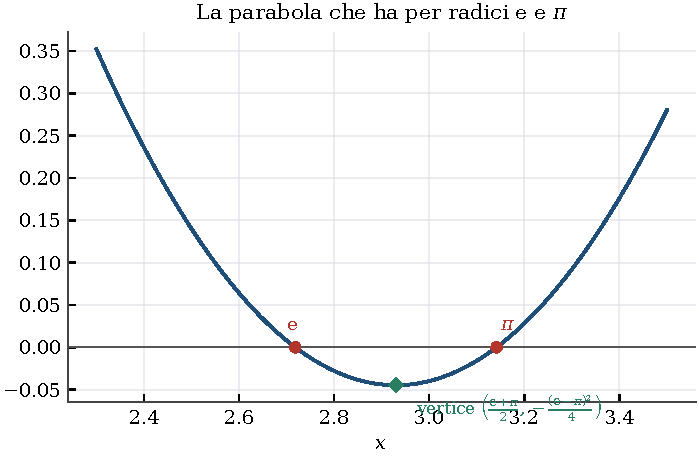
\includegraphics[width=0.86\linewidth]{../figures/e_parabola.pdf}
  \caption{La parabola $x^2-(\pi+\mathrm{e})x+\pi\mathrm{e}$. L'area fra la curva e l'asse, fra le due radici, vale $(\pi-\mathrm{e})^3/3!$ percorsa da $\pi$ verso $\mathrm{e}$.}
  \label{fig:e_parabola}
\end{figure}
\begin{espr}{46}{User}{}
\[
\frac{\left(\pi - \mathrm{e}\right)^{n}}{n!}
\]
\end{espr}
Il termine generale di una serie esponenziale suggerita dalla forma precedente.

\begin{espr}{47}{Sum(\#46,n)}{}
\[
\sum_{n=0}^{+\infty} \frac{\left(\pi - \mathrm{e}\right)^{n}}{n!}
\]
\end{espr}
La sua somma.

\begin{espr}{48}{Simp(\#47)}{}
\[
\mathrm{e}^{\pi - \mathrm{e}}
\]
\end{espr}
Che vale $\mathrm{e}^{\pi-\mathrm{e}}$.

\begin{espr}{49}{Approx(\#48)}{}
\[
1.527008854
\]
\end{espr}
Circa $1{,}527$.


L'integrale $\#43$ ha un valore notevole. Per un polinomio $(x-a)(x-b)$ si ha sempre $\int_a^b (x-a)(x-b)\,\mathrm{d}x=-\tfrac{(b-a)^3}{6}$, e qui, integrando da $\pi$ a $\mathrm{e}$ cioè nel verso che rovescia il segno, si ottiene esattamente $(\pi-\mathrm{e})^3/3!$. Il fattoriale al denominatore suggerisce il passo successivo, che il quaderno compie subito dopo: se $(\pi-\mathrm{e})^3/3!$ è il termine di indice tre di una serie esponenziale, sommiamo tutti gli altri. Il risultato è $\mathrm{e}^{\pi-\mathrm{e}}\approx 1{,}527$.

\section{Equazioni che legano i due numeri}

Una sequenza di piccole equazioni in cui $\mathrm{e}$ e $\pi$ si scambiano i ruoli di base e di esponente. Le ultime quattro producono un accostamento numerico che vale la pena di seguire.

\begin{espr}{50}{User}{\verificata}
\[
\lim_{n \to \infty} \left(1 + \frac{1}{n}\right)^{n} = \sum_{n=0}^{\infty} \frac{1}{n!}
\]
\end{espr}
Le due definizioni classiche di $\mathrm{e}$ affiancate: il limite e la serie.

\begin{espr}{51}{User}{}
\[
\left(x + \frac{1}{\sum_{n=0}^{\infty} n!}\right)^{\sum_{n=0}^{\infty} n!} = \sum_{n=0}^{\infty} \frac{1}{n!}
\]
\end{espr}
Una scrittura formale in cui compare $\sum n!$, che diverge. È un appunto, non un'identità: il quaderno sta cercando che cosa si possa mettere al posto dell'esponente.

\begin{espr}{52}{User}{}
\[
\left(x + \frac{1}{\pi}\right)^{\pi} = \mathrm{e}
\]
\end{espr}
Un'equazione concreta della stessa famiglia, con $\pi$ all'esponente.

\begin{espr}{53}{Simp(Solve(\#52,x))}{}
\[
x = \mathrm{e}^{\frac{1}{\pi}} - \frac{1}{\pi}
\]
\end{espr}
La sua soluzione.

\begin{espr}{54}{User}{}
\[
\left(1 + \frac{1}{x}\right)^{\pi} = \mathrm{e}
\]
\end{espr}
Variante: l'incognita passa dalla base al denominatore.

\begin{espr}{55}{Simp(Solve(\#54,x))}{}
\[
x = \frac{1}{\mathrm{e}^{\frac{1}{\pi}} - 1}
\]
\end{espr}
La soluzione corrispondente.

\begin{espr}{56}{User}{}
\[
\mathrm{e}^{\pi} - \mathrm{e}^{3}
\]
\end{espr}
Confronto fra $\mathrm{e}^{\pi}$ e $\mathrm{e}^3$, cioè fra $\pi$ e $3$ all'esponente.

\begin{espr}{57}{Approx(\#56)}{}
\[
3.055155709
\]
\end{espr}
Circa $3{,}055$.

\begin{espr}{58}{User}{}
\[
\mathrm{e}^{\pi} - \pi^{\mathrm{e}}
\]
\end{espr}
Il classico confronto fra $\mathrm{e}^{\pi}$ e $\pi^{\mathrm{e}}$.

\begin{espr}{59}{Approx(User)}{}
\[
0.6815349142
\]
\end{espr}
La differenza è positiva: $\mathrm{e}^{\pi}>\pi^{\mathrm{e}}$, come è noto.

\begin{espr}{60}{Simp(Solve(User,x))}{}
\[
x = \pi^{\mathrm{e}}\, \mathrm{e}^{-\pi}
\]
\end{espr}
Il loro rapporto, scritto come soluzione di un'equazione.

\begin{espr}{61}{User}{}
\[
x\, \mathrm{e}^{\pi} - \pi^{\mathrm{e}} = 0
\]
\end{espr}
L'equazione che lo definisce.

\begin{espr}{62}{Approx(\#60)}{}
\[
x = 0.9705482059
\]
\end{espr}
Il rapporto vale $0{,}97055$.

\begin{espr}{63}{User}{}
\[
\mathrm{e}^{\pi} - x\, \pi^{\mathrm{e}} = 0
\]
\end{espr}
L'equazione reciproca.

\begin{espr}{64}{Simp(Solve(\#63,x))}{}
\[
x = \pi^{-\mathrm{e}}\, \mathrm{e}^{\pi}
\]
\end{espr}
Il rapporto inverso.

\begin{espr}{65}{Approx(\#64)}{}
\[
x = 1.030345524
\]
\end{espr}
Che vale $1{,}03035$.

\begin{espr}{66}{User}{}
\[
\frac{\pi^{\mathrm{e}}\, \mathrm{e}^{-\pi} + \pi^{-\mathrm{e}}\, \mathrm{e}^{\pi}}{2}
\]
\end{espr}
La semisomma dei due rapporti: un coseno iperbolico.

\begin{espr}{67}{Approx(User)}{}
\[
1.000446865
\]
\end{espr}
Vale $1{,}000447$, cioè quasi esattamente uno.

\begin{espr}{68}{User}{}
\[
\frac{-\pi^{\mathrm{e}}\, \mathrm{e}^{-\pi} + \pi^{-\mathrm{e}}\, \mathrm{e}^{\pi}}{2}
\]
\end{espr}
La semidifferenza: il seno iperbolico corrispondente.

\begin{espr}{69}{Approx(\#68)}{}
\[
0.02989865915
\]
\end{espr}
Vale $0{,}0298987$. Da confrontare con il capitolo~\ref{cap:sin-cos}.


Le espressioni $\#66$ e $\#68$ costruiscono la semisomma e la semidifferenza di $\pi^{-\mathrm{e}}\mathrm{e}^{\pi}$ e del suo reciproco. Qui conviene dare un nome alla quantità $k=\pi-\mathrm{e}\ln\pi$, perché $\pi^{-\mathrm{e}}\mathrm{e}^{\pi}=\mathrm{e}^{\pi-\mathrm{e}\ln\pi}=\mathrm{e}^{k}$: le due espressioni sono allora, esattamente, $\cosh k$ e $\sinh k$.

Questo spiega il valore $0{,}029898659\ldots$ della riga $\#69$, e spiega perché somigli tanto a $k=0{,}029894206\ldots$ senza coincidervi: $\sinh k-k=k^3/6\approx 4{,}45\cdot10^{-6}$, che è esattamente lo scarto osservato. Non è una coincidenza numerica ma un'identità, e il quaderno \dfw{sin-cos.dfw} del gennaio precedente (capitolo~\ref{cap:sin-cos}) la sviluppa per intero: là si scopre che $k$ è la pulsazione di un intero sistema di funzioni iperboliche costruito su $\pi$ ed $\mathrm{e}$.

\section{Una successione che converge molto più in fretta}

Ritorno al tema centrale, con un'idea nuova: sommare $n^{-k}$ per $k$ da $0$ a $n$, ed elevare alla $n$.

\begin{espr}{70}{User}{}
\[
\lim_{n \to \infty} \left(\sum_{k=0}^{n} \frac{1}{n^{k}}\right)^{n}
\]
\end{espr}
La successione più rapida: somma di $n^{-k}$ per $k$ fino a $n$, elevata a $n$.

\begin{espr}{71}{Simp(User)}{}
\[
1
\]
\end{espr}
\begin{espr}{72}{User}{}
\[
\lim_{n \to 9999999} \left(\sum_{k=0}^{n} \frac{1}{n^{k}}\right)^{n}
\]
\end{espr}
Valutata in $n=10^7-1$.

\begin{espr}{73}{Approx(\#72)}{}
\[
2.718281964
\]
\end{espr}
Il risultato ha sette cifre esatte di $\mathrm{e}$.

\begin{espr}{74}{User}{}
\[
\lim_{n \to 9999999} \left(\sum_{k=0}^{n} \frac{1}{n^{k}}\right)^{n} - \mathrm{e}
\]
\end{espr}
La differenza dal valore vero.

\begin{espr}{75}{Approx(\#74)}{}
\[
1.359141174 \cdot 10^{-7}
\]
\end{espr}
Poco più di un decimilionesimo.

\begin{figure}[htbp]
  \centering
  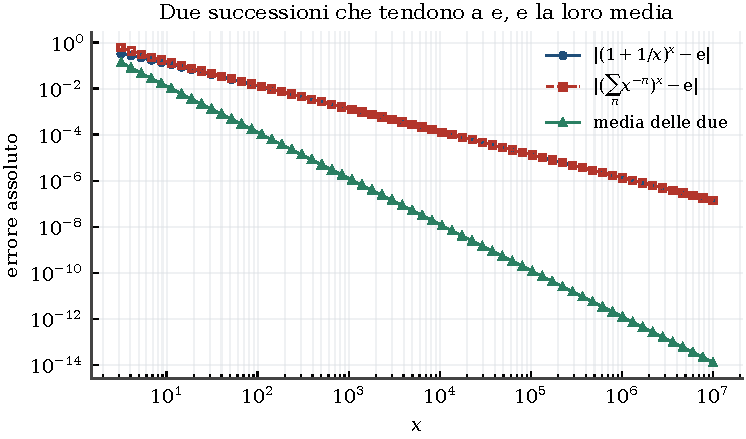
\includegraphics[width=0.86\linewidth]{../figures/e_convergenza.pdf}
  \caption{Errore assoluto delle due successioni al variare di $x$, in scala doppiamente logaritmica. La successione classica scende con pendenza $-1$; quella costruita sulla serie geometrica è di gran lunga più rapida.}
  \label{fig:e_convergenza}
\end{figure}
\begin{espr}{76}{User}{}
\[
\sum_{n=0}^{\infty} \left(\frac{1}{x}\right)^{n} = \frac{x}{x - 1}
\]
\end{espr}
La somma della serie geometrica in forma chiusa.

\begin{espr}{77}{User}{\verificata}
\[
\lim_{x \to +\infty} \left(\frac{x}{x - 1}\right)^{x} = \mathrm{e}
\]
\end{espr}
Il limite per $x\to+\infty$ vale $\mathrm{e}$.

\begin{espr}{78}{User}{\verificata}
\[
\lim_{x \to -\infty} \left(\frac{x}{x - 1}\right)^{x} = \mathrm{e}
\]
\end{espr}
E anche per $x\to-\infty$: la funzione $\left(\tfrac{x}{x-1}\right)^x$ tende a $\mathrm{e}$ da entrambe le parti.

\begin{espr}{79}{User}{}
\[
\left(1 + \frac{1}{x}\right)^{x}
\]
\end{espr}
La successione classica, per confronto.

\begin{espr}{80}{User}{\verificata}
\[
\lim_{x \to -\infty} \left(1 + \frac{1}{x}\right)^{x} = \mathrm{e}
\]
\end{espr}
Che ha la stessa proprietà: il limite da $-\infty$ è ancora $\mathrm{e}$.

\begin{espr}{81}{User}{\verificata}
\[
\lim_{x \to +\infty} \left(\sum_{n=0}^{\infty} \left(\frac{1}{x}\right)^{n}\right)^{x} = \mathrm{e}
\]
\end{espr}
L'equivalenza fra le due scritture.

\begin{espr}{82}{User}{\verificata}
\[
\lim_{x \to +\infty} \left(\sum_{n=0}^{\infty} \left(\frac{1}{x}\right)^{n}\right)^{x} = \sum_{n=0}^{+\infty} \frac{1}{n!}
\]
\end{espr}
E il collegamento con la serie dei reciproci dei fattoriali: tre definizioni in una riga.


Il confronto numerico è impietoso per la definizione classica. La successione $\left(1+\tfrac1n\right)^n$ converge come $1/n$: con $n=10^7$ dà appena sette cifre corrette. La successione $\left(\sum_k n^{-k}\right)^n$ commette invece un errore di $1{,}36\cdot10^{-7}$ allo stesso $n$ — e la differenza si vede meglio nel grafico che nei numeri.

\section{Dal reale al complesso}

L'ultima sezione è la più bella. Si sostituisce $x$ con $\mathrm{i}x$ nella definizione generale e si guarda dove va a finire il limite.

\begin{espr}{83}{User}{\verificata}
\[
\sum_{n=0}^{\infty} \left(\frac{x}{k}\right)^{n} = \frac{k}{k - x}
\]
\end{espr}
Si generalizza introducendo un numeratore $x$: la serie geometrica di ragione $x/k$.

\begin{espr}{84}{User}{\verificata}
\[
\lim_{k \to -\infty} \left(1 + \frac{x}{k}\right)^{k} = \mathrm{e}^{x}
\]
\end{espr}
Il limite diventa $\mathrm{e}^x$, da sinistra...

\begin{espr}{85}{User}{\verificata}
\[
\lim_{k \to +\infty} \left(1 + \frac{x}{k}\right)^{k} = \mathrm{e}^{x}
\]
\end{espr}
...e da destra.

\begin{espr}{86}{User}{\verificata}
\[
\lim_{k \to +\infty} \left(\sum_{n=0}^{\infty} \left(\frac{x}{k}\right)^{n}\right)^{k} = \mathrm{e}^{x}
\]
\end{espr}
Lo stesso con la serie al posto del binomio.

\begin{espr}{87}{User}{\verificata}
\[
\lim_{k \to +\infty} \left(\sum_{n=0}^{+\infty} \frac{x^{n}}{k^{n}}\right)^{k} = \sum_{n=0}^{+\infty} \frac{x^{n}}{n!} = \mathrm{e}^{x}
\]
\end{espr}
Tre scritture equivalenti di $\mathrm{e}^x$: limite, serie di potenze, e la loro identificazione.

\begin{espr}{88}{User}{}
\[
\lim_{x \to +\infty} \left(1 + \frac{2\, \mathrm{i}\, \pi}{x}\right)^{x} = 1
\]
\end{espr}
Primo caso complesso: $z=2\mathrm{i}\pi$ dà $1$, cioè un giro completo.

\begin{espr}{89}{User}{\verificata}
\[
\lim_{x \to +\infty} \left(1 + \frac{\mathrm{i}\, \pi}{x}\right)^{x} = -1
\]
\end{espr}
$z=\mathrm{i}\pi$ dà $-1$: è l'identità di Eulero, ottenuta come limite di una successione reale di numeri complessi.

\begin{espr}{90}{User}{\verificata}
\[
\lim_{x \to +\infty} \left(1 + \frac{\frac{\mathrm{i}\, \pi}{2}}{x}\right)^{x} = \mathrm{i}
\]
\end{espr}
$z=\mathrm{i}\pi/2$ dà $\mathrm{i}$: un quarto di giro.

\begin{espr}{91}{User}{\verificata}
\[
\lim_{k \to +\infty} \left(1 + \frac{\mathrm{i}\, x}{k}\right)^{k} = \mathrm{e}^{\mathrm{i}\, x}
\]
\end{espr}
Il caso generale.

\begin{espr}{92}{User}{\verificata}
\[
\lim_{k \to +\infty} \left(1 + \frac{\mathrm{i}\, x}{k}\right)^{k} = \cos\!\left(x\right) + \mathrm{i}\, \sin\!\left(x\right)
\]
\end{espr}
E la sua lettura trigonometrica. La formula di Eulero compare qui, in fondo, come conclusione di un percorso e non come punto di partenza.

\begin{espr}{93}{User}{}
\[
\lim_{x \to +\infty} \left(\left(1 + \frac{\mathrm{i}\, \pi}{x}\right)^{x} + \left(1 + \frac{2\, \mathrm{i}\, \pi}{x}\right)^{x}\right) = 0
\]
\end{espr}
La somma dei casi $\pi$ e $2\pi$: $-1+1=0$.


Le espressioni da $\#88$ a $\#92$ sono la formula di Eulero ricostruita per via elementare. Se $\left(1+\tfrac{z}{k}\right)^k\to\mathrm{e}^z$, allora ponendo $z=\mathrm{i}\pi$ si ottiene $-1$, ponendo $z=2\mathrm{i}\pi$ si ottiene $1$, ponendo $z=\mathrm{i}\pi/2$ si ottiene $\mathrm{i}$. Sono i tre valori che la funzione esponenziale assume ai quarti di giro, ricavati senza mai scrivere $\mathrm{e}^{\mathrm{i}\theta}=\cos\theta+\mathrm{i}\sin\theta$ — che compare solo alla riga $\#92$, come conclusione e non come premessa. L'ultima espressione somma i casi $\pi$ e $2\pi$ e ottiene zero: $-1+1$.

\section*{In sintesi}
\addcontentsline{toc}{section}{In sintesi}

Il filo che tiene insieme novantatré espressioni è una domanda sola: che cosa, nella definizione $\left(1+\tfrac1x\right)^x$, è essenziale e che cosa è accessorio? La risposta che il quaderno costruisce per prove successive è che conta solo il termine di ordine $1/x$ nella base: tutto ciò che decresce più in fretta è irrilevante, tutto ciò che decresce più lentamente è fatale. Una volta capito questo, sostituire $1$ con $\mathrm{i}x$ è un passo naturale — e la formula di Eulero arriva come corollario.

